%\title{relatório LP}
%----------------------------------------------------------------------------------------
%	PACKAGES AND OTHER DOCUMENT CONFIGURATIONS
%----------------------------------------------------------------------------------------

\makeindex
\documentclass[a4paper,12pt,headings=small]{article}
\usepackage[portuguese]{babel}
\usepackage[export]{adjustbox}
\usepackage[utf8x]{inputenc}
\usepackage{amsmath}
\usepackage{graphicx}
\usepackage{hyperref}
\usepackage{url}
\usepackage[colorinlistoftodos]{todonotes}
\usepackage{placeins}
\usepackage{makeidx}
\usepackage[left=2.5cm,right=2.5cm,top=2.5cm,bottom=2.5cm,a4paper]{geometry}
\usepackage{blindtext}
\usepackage{listings}
\usepackage{float}
\setlength\footskip{1cm}

\lstset{
  language=Java,
  showstringspaces=false,
  columns=flexible,
  basicstyle={\small\ttfamily},
  numbers=none,
  stringstyle=\color{mauve},
  breaklines=true,
  breakatwhitespace=true,
  tabsize=4
}

\begin{document}

\begin{titlepage}

\newcommand{\HRule}{\rule{\linewidth}{0.5mm}} % Defines a new command for the horizontal lines, change thickness here

\center % Center everything on the page




 %----------------------------------------------------------------------------------------
%	LOGO SECTION
%----------------------------------------------------------------------------------------

\includegraphics[scale=1]{uelogo.png}\\[0.5cm] 

%----------------------------------------------------------------------------------------
 
%----------------------------------------------------------------------------------------
%	HEADING SECTIONS
%----------------------------------------------------------------------------------------

\textsc{\Large Linguagens de Programação}\\[1cm]


%----------------------------------------------------------------------------------------
%	TITLE SECTION
%----------------------------------------------------------------------------------------

\HRule \\[0.4cm]
{ \huge \bfseries Relatório do segundo trabalho prático}\\[0.4cm] 
\HRule \\[1 cm]
 
\includegraphics[scale=0.3]{lp.png}\\[0.5cm] 

%----------------------------------------------------------------------------------------
%	AUTHOR SECTION
%----------------------------------------------------------------------------------------
%
\begin{minipage}{0.4\textwidth}
\begin{flushleft} \large
\emph{Autores:}\\
João \textsc{Marques}, 39996\\
Tiago \textsc{Martinho}, 35735\\
\end{flushleft}
\end{minipage}
~
\begin{minipage}{0.4\textwidth}
\begin{flushright} \large
\emph{Docente:} \\
Teresa \textsc{Gonçalves} \\
\end{flushright}
\end{minipage}\\[2cm]


%----------------------------------------------------------------------------------------
%	DATE SECTION
%----------------------------------------------------------------------------------------
{\large Junho de 2020}\\[1cm]  

\vfill % Fill the rest of the page with whitespace

\end{titlepage}

\newpage
\thispagestyle{empty}
\renewcommand\contentsname{Índice}
\tableofcontents
\newpage

\printindex


\section{Introdução}
\FloatBarrier
No âmbito da unidade curricular de Linguagens de Programação, pretende-se implementar uma máquina \textbf{TISC}. Nesta segunda fase do trabalho pretende-se executar a \textbf{memória de instruções},  que foi desenvolvida na primeira fase do trabalho.\\
Este trabalho foi desenvolvido na linguagem de progamação \textit{Java} usando as biblotecas \textit{JLex} e \textit{JCup}.\\
Esta implementação da máquina \textbf{TISC} tem como objectivo simular e funcinar como um intrepetador de TISC.


\section{Correções do Trabalho Anterior}
\FloatBarrier
Face às melhorias propostas pela docente, a estrutura das classes foi repensada de modo a \textbf{beneficiar} do paradigma \textit{\textbf{Object Oriented}} do \textit{Java}. Deste modo utiliza-se uma interface \textit{Instruction} que define os métodos \textbf{partilhados} por todos os tipos de instruções. Estes métodos são: \textit{execute} e \textit{toString}.


\section{Registos de Ativação}
\FloatBarrier
O \textbf{registo de ativação} (RA) é implementado usando um \textit{vector} de \textit{Integer's}. Nesta implementação não existe uma separação fisíca entre cada RA.\\
Cada registo segue o seguinte diagrama:

\FloatBarrier
\begin{figure}[h]
    \centering
    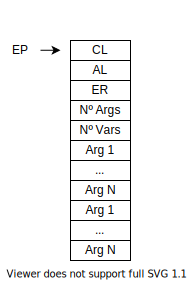
\includegraphics[scale=1]{RA.png}
    \caption{Registo de Ativação}
    \label{fig:my_label}
\end{figure}

\newpage


\section{Estruturas de dados}
\subsection{Memória de Instruções}
\FloatBarrier
Usou-se a mesma estrutura implementada no trabalho anterior, ou seja, um \textit{vector} de instruções. As instruções são entidades polimórficas sendo que existe uma classe diferente para cada. Estas intruções implementam uma interface que define os métodos que devem existir para cada instrução.\\
A memória de instruções é iterada usando o PC (program counter) que face às instruções vai variando de valor.


\subsection{Memória de Execução}
\FloatBarrier
A memória de execução é a zona da máquina TISC que vai guardar os registos de ativação. Foi implementada utilizando um \textit{vector} de \textit{Integer} e fazendo uso de um enviroment pointer. É nesta estrutura onde podemos encontrar os registos de ativação atuais, sendo que o enviroment pointer indica o início do ultimo registo. 

\FloatBarrier
\begin{figure}[h]
    \centering
    \includegraphics[scale=0.8]{exec_memo.jpg}
    \caption{Memória de Execução}
    \label{fig:my_label}
\end{figure}


\subsection{Stack de Avaliação}
\FloatBarrier
Foi usado a classe \textit{Stack} encontrada em \hyperlink{stack}{ \textit{Java.util} } que extende sobre a classe \textit{Vector} propriedades LIFO (\textit{last in first out}) . Esta stack faz parte das estruturas necessárias para a intrepetação da linguaguem TISC.


\subsection{Gestor de Etiquetas}
\FloatBarrier
Para gerir as etiquetas utilizou-se um \hyperlink{hashmap}{ \textit{\textit{HashMap}} } uma vez que se pretende saber o índice
da instrução (PC) a qual a etiqueta corresponde.


\section{Funcionamento das Instruções}
\begin{itemize}
\item \textbf{empilhar} - empilhar um valor na stack de avaliação.
\item \textbf{desempilhar} - desempilha e devolve o valor da stack de avaliação.
\item \textbf{registos} - representa o vector memória de execução.
\item \textbf{FIM} - funciona como o último índice da memória de execução.
\item \textbf{@} - procura o label no gestor de etiquetas e retorna o índice da instrução referente à memória de instruções.
\end{itemize}

\newpage

\subsection{Add}
\begin{lstlisting}
add:
	b = desempilha()
	a = desempilha()
	empilha(a + b)
	PC = PC + 1

\end{lstlisting}

\subsection{Sub}
\begin{lstlisting}
sub:
	b = desempilha()
	a = desempilha()
	empilha(a - b)
	PC = PC + 1

\end{lstlisting}


\subsection{Mult}
\begin{lstlisting}
mult:
	b = desempilha()
	a = desempilha()
	empilha(a * b)
	PC = PC + 1

\end{lstlisting}


\subsection{Div}
\begin{lstlisting}
div:
	b = desempilha()
	a = desempilha()
	empilha(a / b)
	PC = PC + 1

\end{lstlisting}


\subsection{Mod}
\begin{lstlisting}
mod:
	b = desempilha()
	a = desempilha()
	empilha(a % b)
	PC = PC + 1

\end{lstlisting}


\subsection{Exp}
\begin{lstlisting}
exp:
	b = desempilha()
	a = desempilha()
	empilha(a ^ b)
	PC = PC + 1

\end{lstlisting}

\newpage

\subsection{Push int}
\begin{lstlisting}
push_int (integer1):
	empilha(integer1)
	PC = PC + 1

\end{lstlisting}


\subsection{Push var}

\begin{lstlisting}
push_var (integer1, integer2):
	temp = EP	
	
	for i <- 0 to integer1	do
		AL = temp + 1
		temp = registos[AL]
	
	numero_argumentos = registos[temp + 3]
	
	posicao_variavel = temp + 4 + numero_argumentos + integer2
	
	empilha(registos[posicao_variavel])	
	
	PC = PC + 1

\end{lstlisting}


\subsection{Store var}
\begin{lstlisting}
store_var (integer1, integer2):
	temp = EP
	
	valor = desempilha()
	
	for i <- 0 to integer1	do
		AL = temp + 1
		temp = registos[AL]
	
	numero_argumentos = registos[temp + 3]
	
	posicao_variavel = temp + 4 + numero_argumentos + integer2
	
	registos[posicao_variavel] = valor
	
	PC = PC + 1

\end{lstlisting}

\newpage

\subsection{Push arg}
\begin{lstlisting}
push_arg (integer1, integer2):
	temp = EP	
	
	for i <- 0 to integer1	do
		AL = temp + 1
		temp = registos[AL]
	
	posicao_variavel = temp + 4 + integer2
	
	empilha(registos[posicao_variavel])	
	
	PC = PC + 1

\end{lstlisting}


\subsection{Store arg}
\begin{lstlisting}
store_arg (integer1, integer2):
	temp = EP	
	
	valor = desempilha()
	
	for i <- 0 to integer1	do
		AL = temp + 1
		temp = registos[AL]
	
	posicao_variavel = temp + 4 + integer2
	
	registos[posicao_variavel] = valor
	
	PC = PC + 1

\end{lstlisting}


\subsection{Set arg}
\begin{lstlisting}
set_arg (integer1):
	valor = desempilha()
	
	registos[FIM] = valor
	
	PC = PC + 1

\end{lstlisting}

\newpage

\subsection{Call}
\begin{lstlisting}
call (integer1, label):

	// trata do novo EP
	
	registos[FIM] = EP

	EP_antigo = EP
	
	EP = FIM
	
	// trata do novo AL
	
	if integer1 < 0 then
		novo_AL = registos[EP]
		
	if integer1 = 0 then
		novo_AL = registos(EP_antigo)
		
	if integer1 > 0 then
		EP_anterior = registos(EP_antigo)
		
		for i <- 1 to integer1 then
			novo_AL = registos[EP_anterior + 1]
			EP_anterior = novo_AL
			
	registos[FIM] = novo_AL
		
	PC = @label

\end{lstlisting}

\newpage

\subsection{Locals}
\begin{lstlisting}
locals (integer1, integer2):

	registos[FIM] = integer1
	registos[FIM] = integer2
	
	// receber argumentos
	
	inicio_bloco = registos[EP]
	
	// nao valido para a primeira chamada
	
	numero_argumentos_ant = registos[inicio_bloco + 3]
	numero_variaveis_ant = registos[inicio_bloco + 4]
	
	argumento = inicio_bloco + numero_argumentos_ant +
		numero_variaveis_ant
		
	for i <- 0 to integer1 do
		registos[FIM] = registos[argumento]
		delete(registos[argumento])
		EP = EP - 1
	
	for int k <- 0 to integer2 do
		registos[k] = NIL
		
	PC = PC + 1

\end{lstlisting}


\subsection{Return}
\begin{lstlisting}
return:

	EP_antigo = EP
	PC = registos[EP + 2]
	EP = registos[EP]
	
	// apaga registo que ja nao existe	
	
	while EP_antigo != FIM + 1 do
		delete(registos[EP_antigo])
		
\end{lstlisting}

\newpage

\subsection{Jump}
\begin{lstlisting}
jump (label):

	PC = @label
		
\end{lstlisting}


\subsection{Jeq}
\begin{lstlisting}
jeq (label):

	b = desempilha()
	a = desempilha()
	
	if a = b then
		PC = @label
		
	else
		PC = PC + 1	
	
\end{lstlisting}


\subsection{Jlt}
\begin{lstlisting}
jlt (label):

	b = desempilha()
	a = desempilha()
	
	if a < b then
		PC = @label
		
	else
		PC = PC + 1	
	
\end{lstlisting}

\newpage

\subsection{Print}
\begin{lstlisting}
print:

	a = desempilha()
	
	print(a)
	
\end{lstlisting}


\subsection{Print str}
\begin{lstlisting}
print_str (string):

	print(string)
	
\end{lstlisting}


\subsection{Print nl}
\begin{lstlisting}
print_nl:
	print(\n)
	
\end{lstlisting}

\newpage

\section{Execução}
\FloatBarrier
Para compilar e executar deve-se utilizar o \textit{Makefile} fazendo \textit{make} e \textit{make run} respectivamente.\\
Caso se queria ver as mensagens de debug deve-se utilizar os argumentos da função \textit{executa} da máquina TISC. Este debug permite ver as instruções que estão a ser executadas, a memória de execução e a pilha de avaliação.


\section{Referências}
\hypertarget{stack}{[1]}    \url{https://docs.oracle.com/javase/7/docs/api/java/util/Stack.html}\\
\hypertarget{hashmap}{[2]}    \url{https://docs.oracle.com/javase/8/docs/api/java/util/HashMap.html}

\end{document}


